\documentclass[journal]{IEEEtran}
\usepackage{verbatim, xspace, algorithm,algpseudocode, units, graphicx, amsmath,amssymb,url,setspace, array, multirow,caption,color, ntheorem,unicode,subfig}
\usepackage[normalem]{ulem}
\usepackage{aecompl}

\newtheorem{mydef}{Definition}
\newtheorem{mythrm}{Theorem}
\newtheorem{myprf}{Proof}
\theoremsymbol{$\square$}

\newcommand{\etal}{et al.\@\xspace}


\begin{document}
\title{Hierarchical Context-Aware Anomaly Diagnosis in Large-Scale PV System Using SCADA data (OUTLINE)}
\maketitle

\begin{abstract}
Accurate anomaly diagnosis is essential for reducing operation and maintenance (O\&M) cost, while improving safety and reliability of a large-scale photovoltaic (PV) system. This paper presents a hierarchical context-aware anomaly diagnosis approach in PV system, which requires no additional hardware support beyond widely adopted supervisory control and data acquisition (SCADA) system. The proposed approach aims to implement accuracy anomaly diagnosis based on unsupervised machine learning techniques for strings of a PV system. It is motivated from strings  patterns that are related with their electrical characteristics in space and time.  The spatial and temporal distribution of different strings provides rich indications for understanding theirs operation patterns so as to implement anomaly diagnosis. Evaluations using a 40MW PV system located in Northeast China reveal that the proposed diagnosis approach can implement string-level anomaly diagnosis with accuracies higher than \textcolor[rgb]{1,0,0}{97\%} on a daily basis, which satisfy the solar farm requirements.
% The study of fault diagnosis technique plays an important role in the development of cost-effective fault diagnosis techniques in PV system, which can prevent an incipient failure thus to improve system?s reliability. 
%This paper focuses on the electro-thermal analysis for fault detection in a photovoltaic (PV) system. Starting from an analysis of the PV system operation and its power losses mechanism, a model that synthesizes the thermal mechanism and PV system principle is developed to study the potential fault in PV system. Applications of the model are demonstrated comparing simulation results and real-world SCADA data analysis. The results show the linearity/nonlinearity of the model temperature rise with solar irradiance/ output power that can effectively indicate a fault? Different temperature rising shows different fault type. (hot spot, shading, soiling, delamination, browning, ???aging????). The method can be applied to diagnose some failure modes which are hard to identify from ?analysis. The developed thermal model can play a central role for the purpose of fault diagnosis by deriving relationships between various SCADA signals and revealing changes in the thermophysics of PV system operation.
\end{abstract}

\begin{keywords}
Context-aware, anomaly diagnosis, PV system.
\end{keywords}


\section{Introduction}
\label{sect::intro}
%Sting-level anomaly diagnosis is indeed a key issue: high-frequency, hard detection, extremely damaging.
Photovoltaic (PV) systems, as one of mature technologies for power production from renewable energy sources, has shown a rapid growth over the past years. However, as shown in recent studies [?], the large-scale PV system incurs ever-increasing risks of operation and maintenance (O\&M) concerns. How to minimize O\&M cost, while improve safety and reliability of a large-scale photovoltaic (PV) system has become major concerns for PV plants. Strings, as one of the most important part in PV system, and the failures of which occurs at a high frequency and is hard to implement diagnosis for the large area of a large-scale PV system. More seriously, these failures is extremely damaging to a PV system, such as fire hazards [?]. To this end, the goal of this study is to develop effective diagnosis approach for large-scale PV system on string-level basis to reduce O\&M cost, while improve safety and reliability of PV systems. 

%Current works did not address the issue completely: high-cost, false alarm, based on simulation not on practicing(?).
Recent research work has tackled the anomaly diagnosis for PV systems. High-cost is the primary limiting factor to one of the existing solutions [?], as expensive, extra sensing devices are required [?]. For instance, Radu~\etal [online fault detection in pv systems] developed an online fault detection method by developing a model to analyze solar irradiance and PV panel temperature provided by extra a sunshine pyranometer (SPN) and temperature transducers on each PV panel. Due to the high installation and maintenance cost, to date, the adoption rate of extra sensing devices has been low in existing PV plants. Compared with model-based methods, data-driven methods do not rely on expensive extra devices, but utilize the SCADA system, which is considered as a standard installation equipment. These methods, unfortunately, either have a high false alarm rate [hampel identifier], or are not computation-efficient [LOF] for large-scale PV systems. In addition, there are still some hybrid methods combining model-based and data-driven methods that implement performance evaluation of PV systems. However, on the one hand, these methods are based on simulation environment and lack practice application [?]. On the other hand, these methods usually localize on a system-level anomaly detection, which can not conduct anomaly isolation, identification and classification on a fine-grained anomaly diagnosis for offering better scheduling repair, such as string-level. 

%our work
This work aims to tackle string-level anomaly diagnosis problem for a large-scale PV system using SCADA data. The proposed work is based on a hierarchical context-aware anomaly diagnosis model. First, our model is based on a data-driven method such that its implementation does not require any redundant purpose-built sensing device. Second, the hierarchical model ensures the combination between local context and global context, which can minimize the ambient effect so as to reduce false alarm effectively while achieve more accuracy diagnosis rate. Most importantly, the proposed approach is developed and validated using real world 40MW PV plants data (8199 strings over 1 year). Experimental results demonstrate that the proposed approach can perform accurate diagnosis for string-level anomaly on a daily basis, which is sufficient to schedule maintenances activities. 

In this paper, our key contributions are as follows:
\begin{enumerate}
\item We are the first to identify and analyze which contexts can be exploited for string operation patterns recognition and anomaly diagnosis using SCADA system theoretically. Our studies show that statistical information in temporal and spatial, based on string-level, which can be adopted to infer strings operation patterns on a daily basis; 
\item A hierachical context-aware anomaly diagnosis method is proposed to automatic identify strings operating state, in which spatio-temporal information are considered in a Gaussian Mixture Model (GMM) while combining unsupervised machine learning algorithm to achieve accurate anomaly diagnosis; 
\item The proposed approach is evaluated using a real-world PV plant data collected by SCADA system, and experimental results demonstrate that the proposed diagnosis method can accurately infer strings state with accuracies higher than \textcolor[rgb]{1,0,0}{97\%}; 
\end{enumerate}

The rest of this paper is organized as follows.
Section~\ref{sctn:related} outlines the current related works.
Section~\ref{sctn:chllngs} discusses the challenges in anomaly diagnosis of PV systems.
Section~\ref{sctn:mdlfmlt} provides the model formulation.
Section~\ref{sctn:model} presents the hierarchical context-aware anomaly diagnosis model in detail.
Experimental results are presented in Section~\ref{sctn:Exp}.
Finally, we conclude this work in Section~\ref{sctn:cnclusn}.

\section{Related Work}
\label{sctn:related}
Existing anomaly diagnosis methods for PV systems can be categorized into three classes: model-based approaches [?], data-driven approaches [?] and hybrid approaches [?].

Model-based approaches typically use an explicit mathematical model to reason the causality of the components inherent operation principle. A significant difference between the model output and measured signal was considered an anomaly. ...... In summary, these model-based approaches typically require operation features that can only be collected by redundancy sensing device, which can not be supported by SCADA system.

The data-driven methods utilizes statistical approaches and machine learning techniques, which learn models directly from the data. ...... On the one hand, it requires large amount of data and numerous examples to develop an accurate model. In practice, it is very expensive and difficult to obtain labelled data to establish an accurate model.

The hybrid approaches that combines model-based approaches with data-driven approaches has been widely studied. ...... Overall, these hybrid approaches usually localize on a system-level anomaly detection, which can not conduct anomaly diagnosis on a fine-grained anomaly diagnosis for offering better scheduling repair, such as string-level. 

\section{Challenges}
\label{sctn:chllngs}
The primary challenges to tackle anomaly diagnosis has always been the exploration of a set of meaningful and actionable features to indicate the hidden relationship among limited few signals collected by SCADA system.

Nevertheless, SCADA system provides information which can potentially reveal strings operations states.

The diversity of anomaly in string-level poses another challenge in diagnosis methods. Most current approaches are built on case-by-case basis that can not be possible to conduct a general anomaly detection .

The lack of true labelled data is is another challenges we need to consider. It is very expensive and difficult to obtain true labelled data.

\section{MODEL FORMULATION}
\label{sctn:mdlfmlt}
\subsection{Preprocessing}
Current is the major concern. However, currents show high fluctuation. An instantaneous current may not decide whether there is an anomaly is a string.
\begin{table}[!h]
\scriptsize
\caption{PARAMETERS IN OUR REAL WORLD PV SYSTEM}
 \label{sctn:model}
\centering
\begin{tabular}{| c | c | c  | c |}
\hline
  Parameters              & Symbol  & Value     \\
\hline
Area of the PV module         & A  & 1.941 m$^2$        \\
\hline
Maximum Power       & P$_{mppt}$  & 300 W    \\
\hline
Maximum Power Voltage       & V$_{mppt}$  &  36.50 V  \\
\hline
Maximum Power Current       & I$_{mppt}$  &  8.22 A \\
\hline
Open-circuit voltage        & V$_{OC}$  &  45.3 V  \\
\hline
Short-circuit Current        & I$_{SC}$  &  8.79 A \\
\hline
The number of series solar cells per module        & N$_{S}$  &    \\
\hline
temperature factor        & $\delta$  & -0.43\%   \\
\hline
Standard Test Conditions Tempture        & T$_{STC}$  & $25^\text{o}$C   \\
\hline
Standard Test Conditions irradiance        & G$_{STC}$  & 1000  W/$m^2$   \\
\hline
conversion efficiency for module        & $\eta_r$  & 15.45\%   \\
\hline
\end{tabular}
\label{tb:RE_Uniform}
\end{table}

%Note than, we choose the solar irradiance is equal or larger than $300w/m^2$ because the sensors error is relatively big in the solar irradiance is less than $300w/m^2$. From Figure~\cite{fig:fig:irrVScpr}, we can figure out the relationship between in-plane solar irradiance and CPR. (THE detail analysis can be seen in [a simple model of pv system])
\subsection{Local Context}
All strings in the same combiner box are supposed to exhibit the similar characteristics. Thus, the local context in the same combine box 

\subsection{Global Context}
In a PV system, most of strings function properly most of the time, and anomaly strings number is relative few to the total number of strings.

\section{PROPOSED HIERARCHICAL CONTEXT-AWARE ANOMALY DIAGNOSIS MODEL}
\label{sctn:mdl}
\subsection{Local Context-Aware Algorithm}
....an algorithm goes here

We can calculate the normal module temperature.
\begin{equation}
\label{eqn:Tcell}
T_{cell}= \frac{f(v)\cdot T_a +G(t) \cdot (\alpha \cdot \tau -\eta_r -\delta \cdot \eta_r \cdot T_{STC})}{f(v)-\delta\cdot \eta_r\cdot G(t)}
\end{equation}

\begin{equation}
\label{eqn:fv}
f(v)=17.1+5.7\cdot v
\end{equation}
Where $v$ is wind speed; $T_a$ is the ambient temperature; $\alpha \cdot \tau =0.9$.
\subsection{Global Context-Aware Algorithm}
....an algorithms goes here

\begin{equation}
\label{eqn:input}
CPR= \frac{PR}{1+\delta \cdot (T_{cell}-T_{STC})}
\end{equation}

\begin{equation}
\label{eqn:pr}
PR=\frac{E(t)_{AC}}{E_{input}}
\end{equation}

\begin{equation}
\label{eqn:input}
E_{input}= \int G(t)\cdot A \cdot \eta_r \cdot dt
\end{equation}

%\begin{figure}[!tb]
%  \centerline{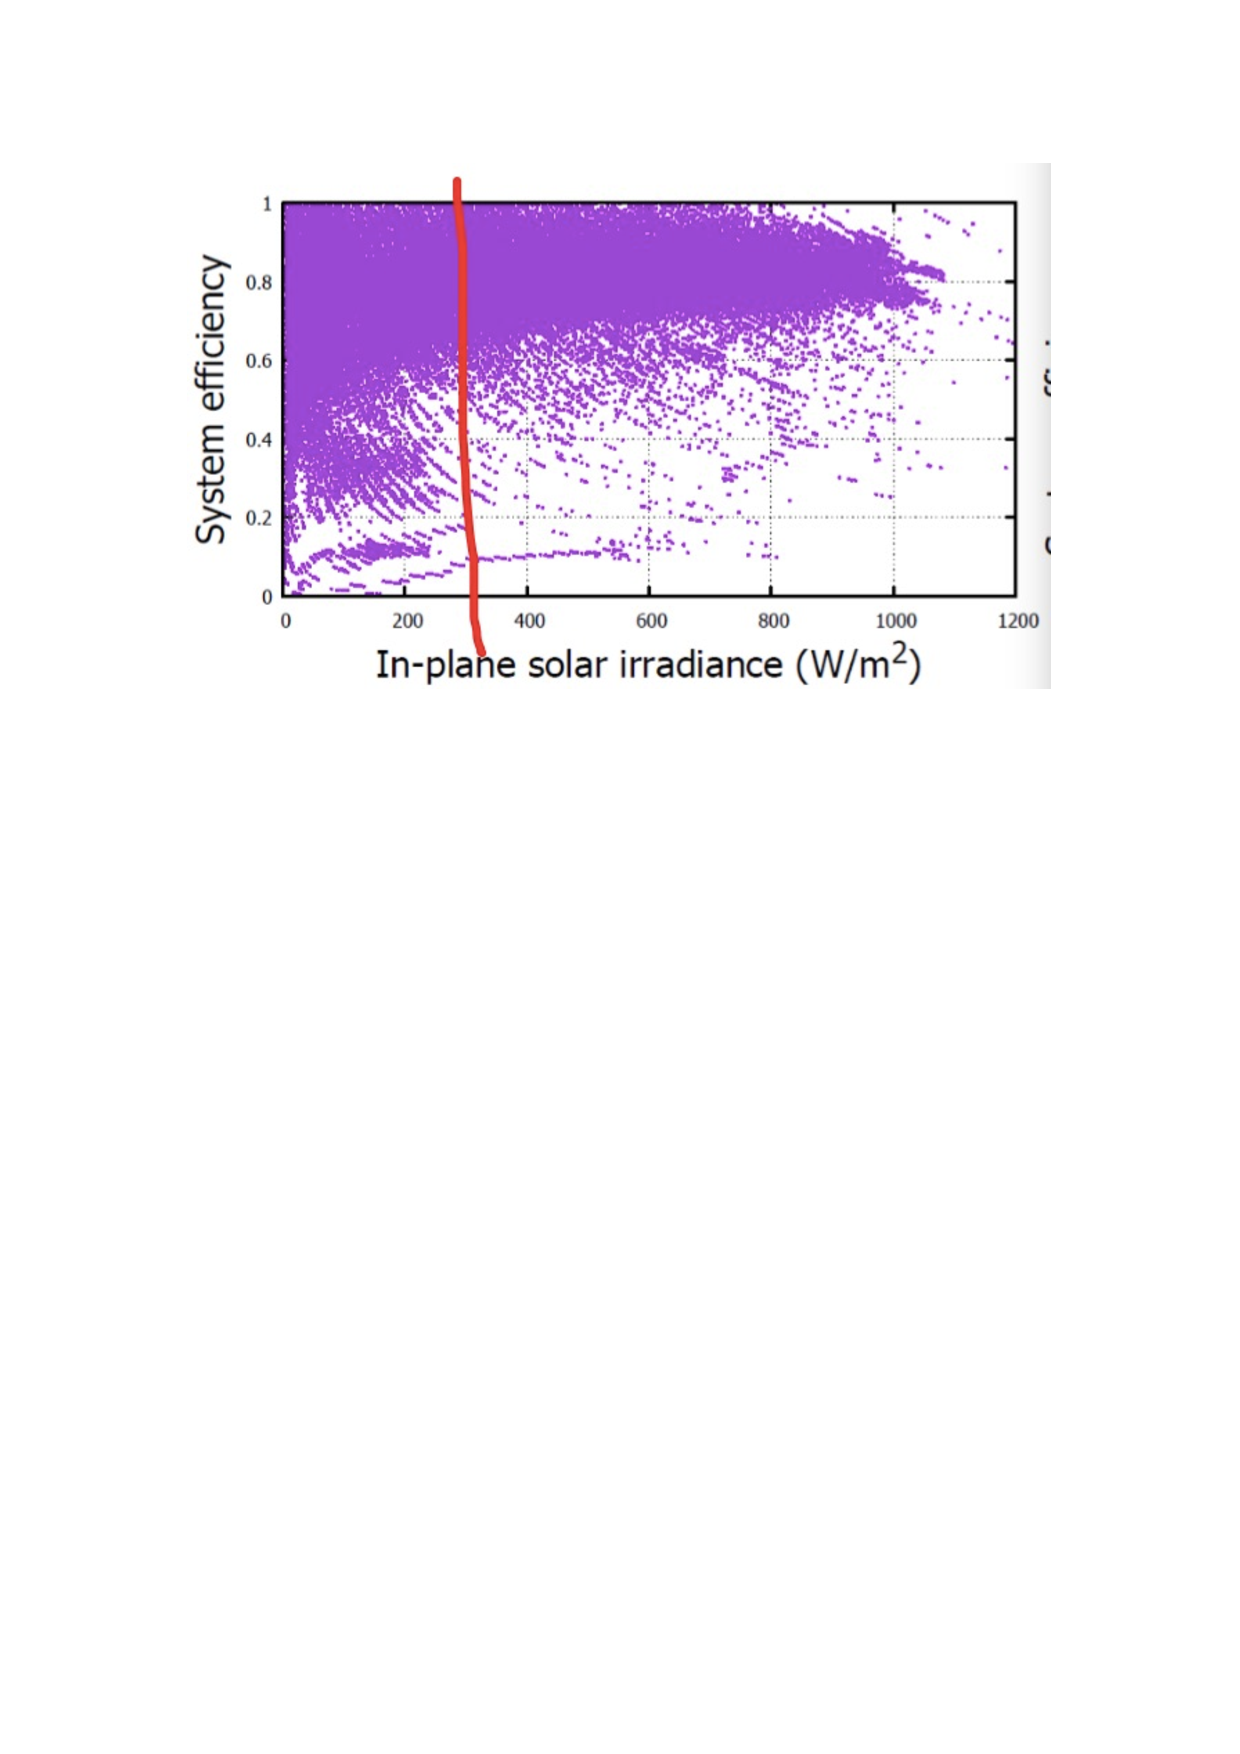
\includegraphics[width=0.45\textwidth]{Figure/irradianceAndCPR.pdf}}
 %   \captionsetup{belowskip=-18pt}
  %\caption{x-minute in-plane solar irradiance to system efficiency values recorded for seven month for a PV system.}
  %\label{fig:irrVScpr}
%\end{figure}
Where $\delta$ is the corrective factor of temperature; $T_cell$ is the module temperature. $T_{STC}$ is the standard temperature; $E(t)_{AC}$ (Wh) is the electrical energy output from combiner box recorded over a time minute period $t$; $G(t)$ is the in-plane solar irradiation received on an unshaded surface of the same location; $A$ (m$^2$) is the area of the PV module; $\eta_r$ is the conversion efficiency of an array.
\subsection{Hierarchical Context-Aware Algorithm}
...an algorithms goes here

\section{EXPERIMENTS AND RESULTS}
 \label{sctn:Exp}
\subsection{Dataset Description and Evaluation Metrics}
There are 74 inverters, 553 combiner boxes, 8199 strings , 131184 modules in a real-world PV system. There are 16 modules in each string. There are 72 cells in each module.
\subsection{Overall Performance}
\subsection{A Case Study}
\section{Conclusion}
\label{sctn:cnclusn}

\bibliographystyle{IEEEtran}
%\bibliography{reference}

\end{document}
%%
%% End of file `elsarticle-template-harv.tex'.
